\chapter{TINJAUAN PUSTAKA DAN KONSEP DASAR SISTEM}

\section{Prinsip Kerja Sistem}
Berdasarkan rumusan masalah yang telah dipaparkan pada bab 1, berikut adalah konsep prinsip kerja sistem yang dicanangkan:
\begin{enumerate}
	\item Terdapat 2 drone dan 1 \textit{Base Station} (BS), masing-masing menggunakan mikrokontroler ESP32 yang berkomunikasi satu sama lain menggunakan JSON \textit{messages} pada jaringan PainlessMesh. Drone 1 disebut sebagai \textit{"sender node"}, dan drone 2 disebut sebagai \textit{"receiver node"}.
	\item ESP32 Drone 1 mengaktifkan modul GPS dan mendata koordinat lokasi, ketinggian terbang drone, dan jumlah satelit yang mendapat \textit{lock}, kemudian menghidupkan LED hijau pada \textit{board}.
	\item Drone 2 mengirimkan permintaan data lokasi kepada drone 1.
	\item Drone 1 mengirimkan data melalui jaringan mesh kepada drone 2. Drone 2 menghidupkan LED hijau setelah menerima data lokasi yang valid.
	\item BS mengirimkan permintaan data pada drone 1 berupa \textit{string} dalam \textit{message}.
	\item Drone 1 mengirimkan data melalui jaringan mesh kepada BS.
	\item BS menampilkan data kepada pengguna melalui \textit{WiFi Access Point} yang dapat diakses dari sebuah \textit{website}. WiFi AP tersebut dibangun menggunakan sebuah board ESP8266 yang menerima data dari board ESP32 yang terhubung dengan jaringan mesh melalui sambungan serial.
\end{enumerate}
\begin{figure}[h]
	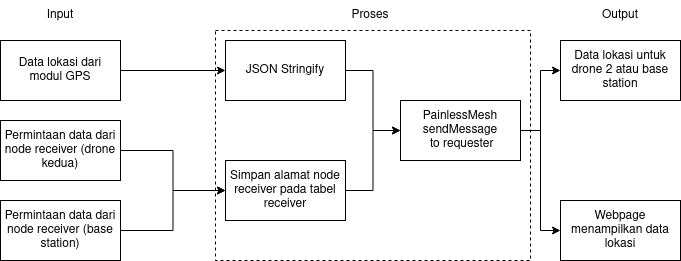
\includegraphics[scale=0.60]{./assets/IOProses}
	\caption{Desain konsep sistem}
\end{figure}
PainlessMesh bekerja menggunakan mode AP-STA pada mikrokontroler ESP32, dimana \textit{board} bekerja sebagai \textit{Wi-Fi Access Point} sekaligus \textit{Wi-Fi Station Mode} untuk membentuk sebuah jaringan mesh. Masing-masing node memiliki sebuah node ID, dan pada aplikasi penelitian ini memiliki penanda sebagai \textit{sender} (node yang mendata lokasi GPS dan mengirimkan data tersebut) dan \textit{receiver} (node yang menerima data lokasi tersebut).

\begin{figure}[h]
	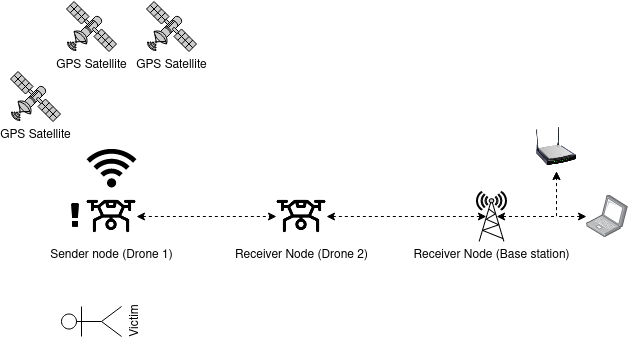
\includegraphics[scale=0.5]{./assets/Diagram Sistem}
	\caption{Diagram sistem}
\end{figure}

Node \textit{sender} memiliki modul GPS yang berkomunikasi dengan satelit untuk mendapatkan data lokasi yang terlampir dalam \textit{NMEA sentences}. Data tersebut kemudian diolah menggunakan \textit{library} TinyGPS++ untuk mengekstraksi data lokasi dari \textit{NMEA sentences} tersebut.

\textit{Sender node} memiliki sebuah \textit{flag} "locationReady" dimana jika nilainya \textit{"true"} maka dapat menerima permintaan data lokasi dari \textit{receiver node}. Kriteria untuk \textit{flag} tersebut memiliki nilai \textit{"true"} adalah telah mendapatkan \textit{lock} satelit minimal 3 dan telah mendapat nilai lintang dan bujur bukan nol.

Akses ke \textit{Base Station} menggunakan sebuah board ESP8266 yang terhubung secara serial dengan board ESP32 yang terhubung dengan jaringan mesh. Konfigurasi ini diperlukan karena limitasi dari board ESP32 yang memiliki koneksi bersamaan maksimum sebanyak 2 (1 dari klien \textit{Access Point}, 1 menjadi klien AP sebagai \textit{Station Mode}), sedangkan PainlessMesh menggunakan kedua mode tersebut untuk mempertahankan jaringan mesh yang dibentuk.

\section{Riset Terkait}
Terdapat beberapa penelitian yang telah dilaksanakan sebelumnya yang terkait dengan tugas akhir ini, yang akan digunakan sebagai dasar atau referensi dalam pengerjaan. Beberapa penelitian terkait dapat dilihat pada tabel 2.1.
\pagebreak
\begin{center}
	\footnotesize
	\captionof{table}{Penelitian terkait}
	\begin{longtable}{|p{0.5cm}|p{2cm}|p{2cm}|p{2cm}|p{2cm}|p{2cm}|}
		\hline
		&\textbf{Judul}&\textbf{Metode}&\textbf{Kesimpulan}&\textbf{Kelebihan}&\textbf{Kekurangan}\\
		\hline
		\cite{santosUseHighMobility2021}&Use of High Mobility Nodes to Improve Connectivity in Wireless Sensor Networks&PainlessMesh-based Opportunistic Mobile Ad Hoc Networks&Menggunakan high mobility nodes berupa drone sebagai messenger data antara cluster sensor dengan server&Penelitian mengimplementasikan metode security berbasis secret-key cryptography. Packet loss antara sensor dan server rendah, hanya 4,48\% pada kondisi terburuk walaupun packet melewati 2 hop.
		&Tidak menguji round-trip delay packet\\
		\hline
		\cite{chiaPerformanceEvaluationESP82662019a}&Performance Evaluation of ESP8266 Mesh Networks&Pengujian one-way delay dan data rate pada jaringan PainlessMesh ESP8266& Jumlah node berkorelasi dengan meningkatnya single hop delay dan menurunnya stabilitas jaringan, serta besar payload menentukan data rate dan korupsi data.&Penelitian menguji dari 2 hingga 16 node sehingga terlihat gambaran kasar stabilitas jaringan PainlessMesh. Kinerja jaringan 2 node memiliki delay 2.49 ms sehingga cukup untuk aplikasi yang tidak terlalu kompleks.&ESP8266 tidak memiliki performa yang cukup untuk mengirimkan dan menerima payload data yang besar. Pengujian data rate dibatasi pada 2 node. \\
		\hline
		\cite{manviImplementingWirelessMesh2020}&Implementing Wireless Mesh Network Topology Between Multiple Wi-Fi Powered Nodes for IoT Systems&Penggunaan 3 node PainlessMesh berbasis ESP32 untuk komunikasi multidirectional output sensor dan input push button&Mesh bersifat self-healing, pada saat terjadi disrupsi maka mesh secara otomatis mengatur diri.&Implementasi 3 node dan arah data bolak balik dapat dilakukan&Tidak ada pengujian jarak jauh\\
		\hline
		\cite{guoDustSensorMonitoring2021}&A dust sensor monitoring system using Wi-Fi mesh network&Implementasi 9 node berbasis ESP32 dan ESP-Mesh untuk monitoring tingkat debu pada suatu ruangan.&Sistem efektif dengan measurement error dibawah 5\%&Mesh dapat berfungsi tanpa intervensi manusia, memiliki sifat self-healing dan auto-configuration.& Jaringan memiliki topologi tree, bukan mesh murni, sehingga jika terjadi gangguan pada node akar maka proses self-heal berjalan lebih lama.\\
		\hline
	\end{longtable}
\end{center}
Berdasarkan penelitian yang telah dilakukan sebelumnya, maka penulis akan membatasi penelitian ke 3 node ESP32, menguji \textit{throughput, packet loss, round-trip delay,} dan \textit{signal strength (dBm)}; serta pengujian jarak antar node terhadap kinerja jaringan. Khusus untuk node base station akan disambungkan dengan sebuah board ESP8266 sebagai HTTP Server untuk koneksi web server yang menampilkan data lokasi dari node \textit{sender}.

\section{\textit{Unmanned Aerial Vehicles}}
UAV adalah sebuah pesawat terbang yang dapat mengudara tanpa awak \cite{lakshminarayananJointNetworkDisaster2015}, dikendalikan secara \textit{remote} atau secara otonom. Salah satu tipe UAV adalah \textit{quadcopter drone}. Pada sistem ini, UAV digunakan sebagai pengirim data lokasi GPS sebagai node \textit{sender}, dan penerima data lokasi GPS sebagai node \textit{receiver}.

\section{\textit{Quadcopter}}
Drone \textit{quadcopter} adalah suatu jenis UAV yang memiliki 4 rotor pada masing-masing sudut. Sama seperti helikopter, \textit{quadcopter} memiliki kemampuan untuk \textit{hover}. Terdapat sepasang rotor yang berputar searah jarum jam dan sepasang rotor yang berputar berlawanan arah jarum jam, sehingga pada kondisi \textit{steady state} total torsi pada \textit{drone} adalah nol. Hal tersebut juga menyebabkan konfigurasi \textit{quadcopter} tidak membutuhkan \textit{tail rotor}. Keempat rotor tersebut juga menghasilkan daya angkat yang besar, sehingga cocok digunakan untuk membawa \textit{payload}.

\section{ESP32}
Pada penelitian ini, ESP32 digunakan sebagai modul komunikasi antar node baik drone maupun base station. Board-board ESP32 dapat dikonfigurasikan menjadi jaringan mesh menggunakan mode APSTA/\textit{Coexistence Mode}, dimana secara bersamaan ESP32 mem-\textit{broadcast} SSID sambil terhubung dengan jaringan lain \cite{WiFiDriverESP32}. 

ESP32 juga mendukung protokol \textit{proprietary} buatan Espressif bernama 802.11 LR \textit{(Long Range)}, dengan jarak hingga 1 km selama ada \textit{line-of-sight} antara \textit{node}. \cite{WiFiDriverESP32}.
\begin{figure}[h]
	\centering
	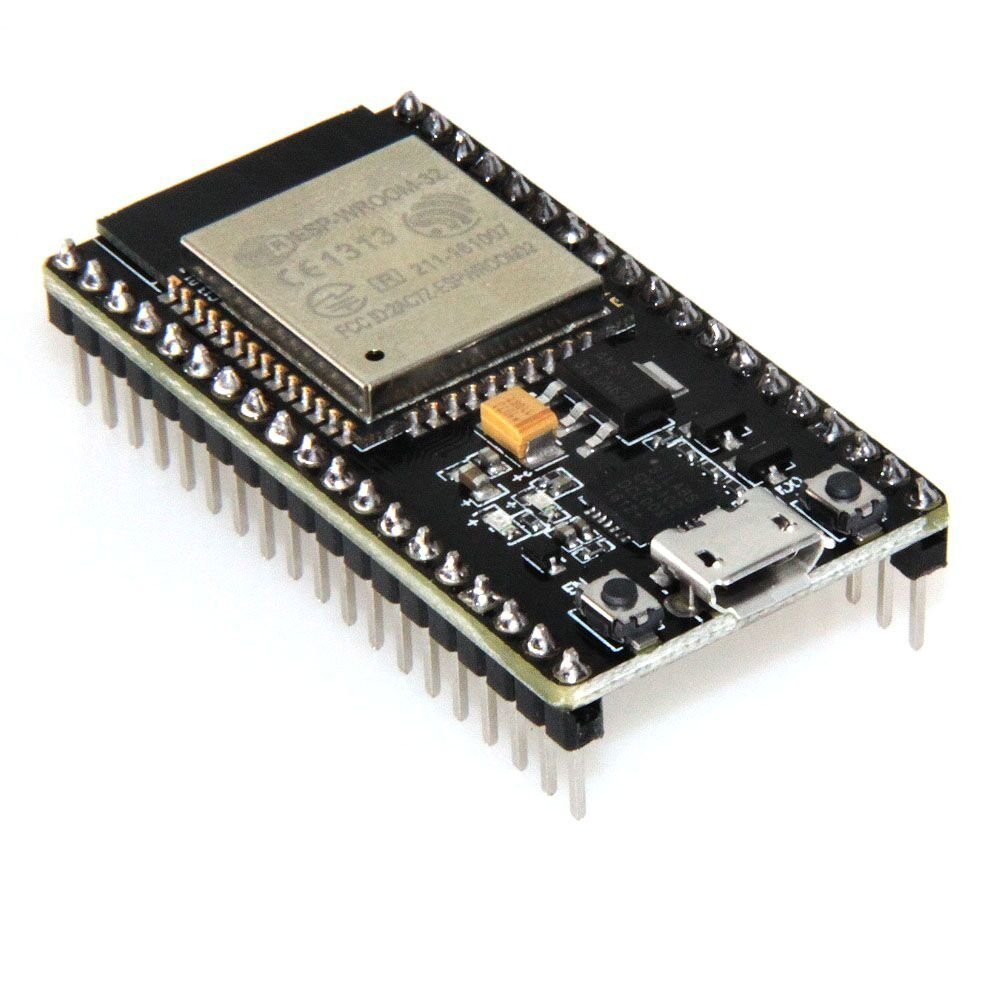
\includegraphics[scale=0.1]{./assets/ESP32}
	\caption{ESP32}
\end{figure}

\section{PainlessMesh}
PainlessMesh merupakan sebuah library yang memudahkan pengguna \textit{board} ESP32 dalam membuat sebuah jaringan mesh ad-hoc berbasis WiFi. Karena batasan dari \textit{board} ESP32, maka jaringan yang dihasilkan merupakan \textit{"pseudo-mesh"} atau mesh yang tidak sempurna, sehingga pada kondisi standar, semua node memiliki kedudukan yang sama dan diatur dalam topologi \textit{tree}.

Jaringan PainlessMesh menggunakan mode APSTA pada board ESP32, dimana setiap board ESP32, disebut dengan "node", berfungsi sebagai WiFi \textit{Access Point} (AP) sekaligus sebagai klien WiFi \textit{Station Mode}. Setiap node berbasis ESP32 dapat memiliki sebanyak 10 klien yang terhubung pada 1 AP, dan dapat terhubung pada AP lainnya sebagai sebuah klien.

\begin{figure}[h]
	\centering
	\includegraphics[scale=0.5]{./assets/painlessmesh}
	\caption{Topologi jaringan PainlessMesh \cite{HomeWikiPainlessMesh}, panah menunjukkan arah koneksi dari klien ke AP}
\end{figure}

Keistimewaan dari library PainlessMesh adalah kemampuannya untuk \textit{autoconfigure}, dimana setiap node dapat memutus sambungan dan menyambung ulang setiap saat, dan jaringan mesh dapat berjalan melalui proses konfigurasi secara otomatis.

\section{JavaScript Object Notation (JSON)}
PainlessMesh menggunakan JavaScript Object Notation untuk setiap pengiriman pesan antar-node dalam jaringan. Penggunaan JSON memudahkan penafsiran \textit{(parsing)} setiap pesan yang diterima untuk kemudian diolah menjadi data yang ditampilkan \cite{MeshProtocolWiki}.

\begin{figure}[h]
	\centering
	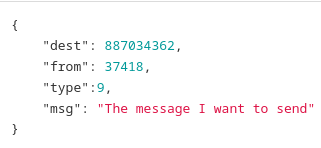
\includegraphics[scale=0.5]{./assets/PainlessMeshJSON}
	\caption{Setiap pesan pada jaringan PainlessMesh menggunakan JSON.}
\end{figure}

Setiap paket data PainlessMesh menggunakan skema JSON untuk menentukan tujuan (dari \textit{key "dest"}), dari mana paket data tersebut berasal (\textit{key "from"}), jenis paket berdasarkan nilai integer pada \textit{key "type"}, serta pesan yang akan dikirim pada \textit{key "msg"}. \newline

\section{GPS NMEA Data}
Modul GPS NEO-6M menghasilkan output serial mentah berupa data NMEA 0183, sebuah standar komunikasi piranti GPS berupa karakter-karakter ASCII yang membentuk kalimat-kalimat NMEA \cite{GPSNMEASentence}.

\begin{figure}[H]
	\centering
	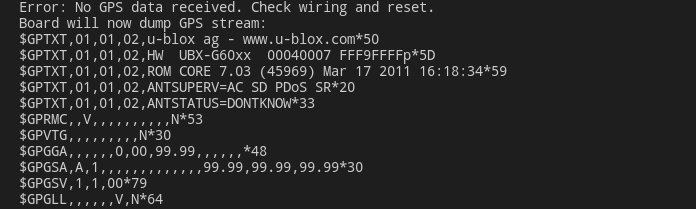
\includegraphics[scale=0.5]{./assets/NMEASentences}
	\caption{Contoh data mentah dari modul GPS NEO-6M berupa data GPS NMEA.}
\end{figure}

\section{Pengukuran Kinerja Jaringan}
\subsection{Round-trip delay}
\textit{Round-trip delay} adalah waktu yang diperlukan untuk sebuah paket data dikirimkan dari node pengirim ke node penerima, ditambah waktu yang diperlukan untuk paket \textit{acknowledge} diterima oleh node pengirim dari node penerima. Pengukuran \textit{round-trip delay} dapat menggunakan fungsi yang sudah diimplementasikan dalam \textit{library} PainlessMesh yakni \verb|painlessMesh::startDelayMeas()|.

Setiap node pada jaringan PainlessMesh memiliki waktu internal yang tersinkronisasi satu sama lain melalui proses \textit{"Time sync"} \cite{MeshProtocolWiki} yang berlangsung secara periodis setiap 10 menit. PainlessMesh menjaga waktu jaringan pada tingkat kepresisian mikrosekon menggunakan fungsi \verb|micros()| pada mikrokontroler ESP32. Kemudian setelah fungsi \verb|startDelayMeas()| dipanggil, maka \textit{round-trip delay} dapat dihitung menggunakan rumus berikut:

\[ t_{round trip} = (t_3 - t_0) - (t_2 - t_1) \]
$t_0$ = waktu internal pada pengirim \textit{delay measurement}\\
$t_1$ = \textit{timestamp} pada saat paket \textit{delay measurement} diterima\\
$t_2$ = \textit{timestamp} pada saat respon terhadap \textit{delay measurement} dikirimkan\\
$t_3$ = \textit{timestamp} pada saat respon diterima oleh pengirim \textit{delay measurement}

\subsection{Throughput}
\textit{Throughput} adalah banyaknya data yang dapat ditransmisikan dalam suatu satuan waktu. Pada penelitian ini, \textit{throughput} dihitung setiap pengiriman paket data, dibandingkan dengan perbedaan \textit{timestamp} antara pengiriman dan penerimaan paket data tersebut.

\[Throughput = \frac{sizeof(packet)}{t_1 - t_0}\]
$t_0$ = waktu internal pada saat pengirim mengirim paket data\\
$t_1$ = \textit{timestamp} pada saat penerima menerima paket data

\subsection{Packet loss}
Packet loss adalah jumlah packet data yang hilang dibandingkan packet data yang berhasil dikirimkan.
\[ Packet Loss = (1 - \frac{p_{TX}}{ack_{RX}})\times 100\%\]
$p_{TX}$ = jumlah packet data yang dikirimkan\\
$ack_{RX}$ = jumlah packet \textit{acknowledge} yang diterima

\begin{figure}[H]
	\centering
	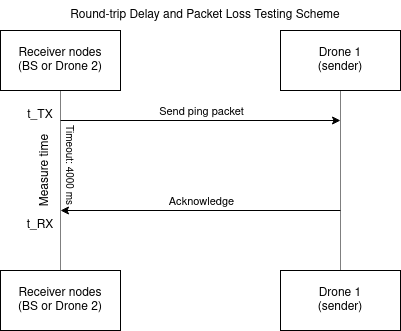
\includegraphics[scale=0.7]{./assets/PingTest}
	\caption{Skema pengujian \textit{round-trip delay} dan \textit{packet loss}}
\end{figure}